\section{The inverse on the whole annulus}
\label{sec:radial-reference-inverse}

Spectral gaps of the individual pieces do not automatically survive
gluing. A homogeneous solution can leave one piece, return through its
neighbour, and satisfy a new matching condition. We must therefore
solve the matching problem for the whole annulus, not just list the
inverses of the pieces. This section does so and completes the proof
of Proposition~\ref{prop:rad-fixed-theorem}.

\subsection{Overview}

Everything is done one frequency at a time. Fix an even frequency $j$
and let $n$ be its band index, $j\in\mathcal I_n$
(Section~\ref{subsec:bands}). At each end the annulus is divided into
three regions (Figure~\ref{fig:frequency-regions}).
\begin{itemize}
\item The \emph{inner region}: the central model, the cells $m<n$ of
 both tails, and the positive intervals between them. All these
 pieces have large action at the frequency $j$, so each is governed by
 its own spectral inverse, and neighbouring pieces are coupled only
 through exponentially small terms.
\item The \emph{outer core} at each end: the join preceding cell $n$
 and cell $n$ itself. Nothing is small here, but the core is a single
 cell: crossing it costs a known finite factor, and the height
 selection of Lemma~\ref{lem:radial-product-selection} keeps the
 matching angle at its entrance above $\delta_n$.
\item The \emph{deep tail} at each end: the cells $m>n$, governed by
 the recurrence of Lemma~\ref{lem:radial-deep-inverse}.
\end{itemize}
The inverse is assembled in four steps: an inner inverse $G_h$ with
zero boundary values at the two entrances of the outer cores
(Section~\ref{subsec:rad-localized-hilbert-assembly}); an outer inverse
$R_o$ at each end, with the natural condition at the endpoint
(Section~\ref{subsec:outer-inverse}); a $2\times2$ linear system for
the two boundary values that remain, one for each end
(Section~\ref{subsec:terminal-matching}); and weighted estimates for
the resulting formula (Section~\ref{subsec:global-estimate}).

One principle organizes the estimates. A correction created at the
transition cell is large: it costs $\delta_n^{-1}$, the transfer
factor $e^{C_o\tau_{n,j}}$ of the core, and coefficient powers. If its
output stays in cell $n$ or beyond, this cost is absorbed by the
coefficient weight allowed in the output norm there. If its output
returns to the interior, it must first cross the positive cap
preceding the transition join, which attenuates it by
$e^{-c\tau_{n-1,j}}$; and $\tau_{n-1,j}/\tau_{n,j}\asymp e^{n}$, so the
attenuation wins.

\begin{figure}[htbp]
\centering
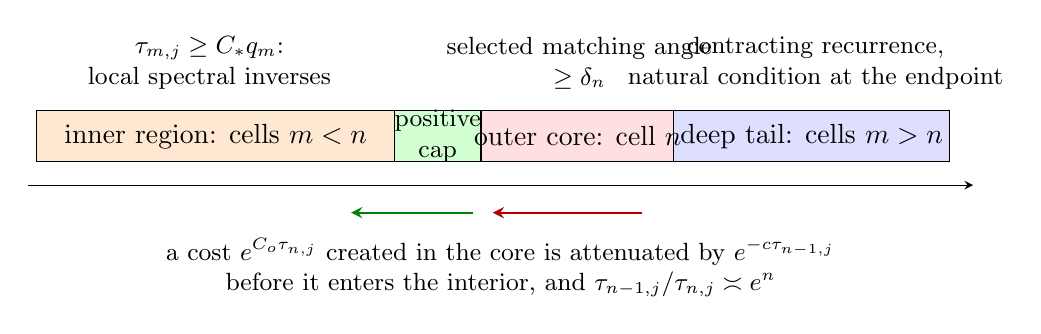
\begin{tikzpicture}[x=1cm,y=1cm,>=stealth]
\draw[->] (0,0)--(12,0);
\draw[fill=orange!18] (.1,.3) rectangle (4.65,.95);
\draw[fill=green!18] (4.65,.3) rectangle (5.75,.95);
\draw[fill=red!12] (5.75,.3) rectangle (8.2,.95);
\draw[fill=blue!13] (8.2,.3) rectangle (11.7,.95);
\node at (2.38,.62) {inner region: cells $m<n$};
\node[align=center,font=\small] at (5.2,.62) {positive\\cap};
\node at (6.98,.62) {outer core: cell $n$};
\node at (9.95,.62) {deep tail: cells $m>n$};
\node[align=center,font=\small] at (2.3,1.55)
 {$\tau_{m,j}\ge C_*q_m$:\\local spectral inverses};
\node[align=center,font=\small] at (7,1.55)
 {selected matching angle\\$\ge\delta_n$};
\node[align=center,font=\small] at (10,1.55)
 {contracting recurrence,\\natural condition at the endpoint};
\draw[->,thick,red!70!black] (7.8,-.35)--(5.9,-.35);
\draw[->,thick,green!50!black] (5.65,-.35)--(4.1,-.35);
\node[align=center,font=\small] at (6,-1.05)
 {a cost $e^{C_o\tau_{n,j}}$ created in the core is attenuated by
  $e^{-c\tau_{n-1,j}}$\\before it enters the interior, and
  $\tau_{n-1,j}/\tau_{n,j}\asymp e^n$};
\end{tikzpicture}
\caption{The decomposition of one end of the annulus at a frequency
$j\in\mathcal I_n$. The other end is treated at the same time. The
position of the division changes with the frequency; the profile is
chosen once.}
\label{fig:frequency-regions}
\end{figure}

\paragraph{Notation of this section.}
We write $w$ for the profile. Estimates are made in the Hilbert space
$L^2(d\mu)$, $d\mu=\varpi\,dr$, with the conventions
\begin{equation}\label{eq:rad-eq-hn1}
 B_j=-\varpi^{-1}L_j,
 \qquad F=-\varpi^{-1}f,\qquad
 \langle u,F\rangle_{L^2(d\mu)}=-\int\overline u\,f\,dr ,
\end{equation}
so that $L_ju=f$ is the same as $B_ju=F$; we also write
$\mathscr H_j=-L_j$. For a border column $k=-\varpi^{-1}g_0$ the
Hilbert adjoint is $k^*u=-\ell_0u$; so after a change of sign of the
scalar equation the bordered operator is symmetric. This convention is
used in all energy identities below. Finite matrices that act on
boundary values are written in sans-serif type when their letter is
also used for a scale ($\mA,\mB,\mK,\mS$). The letters $\lambda$,
$\Lambda$, $\kappa$, $T$, $D$, $E$ have the local meanings stated in
each subsection.

\subsection{Completing the profile while keeping the seed}
\label{subsec:rad-cone-bump-target-match}

We first finish the construction of the profile, in such a way that
the solution of $L_2\phi=0$ is preserved exactly. The device is to
prescribe the solution and to solve for the profile.

\begin{lemma}[Connectors]\label{lem:connector}
On an interval put $y=\log r$ and $w=re^f$, and let $\phi$ be a
nonvanishing function with logarithmic slope
$\mathsf k=\phi_y/\phi$. Then $L_2\phi=0$ is equivalent to
\begin{equation}\label{eq:rad-eq-sp1}
 f_y=\frac{\mathsf k^2+\mathsf k_y-4}{4-\mathsf k},
 \qquad\text{that is,}\qquad
 1+f_y=\frac{rw'}{w}=\frac{\mathsf k^2-\mathsf k+\mathsf k_y}{4-\mathsf k}.
\end{equation}
\end{lemma}

\begin{proof}
In the variable $y$ the equation $r^2L_2\phi=0$ reads
$w\phi_{yy}+(w_y-w)\phi_y-4w_y\phi=0$. Divide by $w\phi$ and use
$\phi_{yy}/\phi=\mathsf k_y+\mathsf k^2$ and $w_y/w=1+f_y$.
\end{proof}

Thus any function $\mathsf k(y)$ with $\mathsf k<4$ and
$\mathsf k^2-\mathsf k+\mathsf k_y>0$ produces, by integrating first
$f_y$ and then $\phi_y=\mathsf k\phi$, a positive interval together
with a solution of $L_2\phi=0$ on it. For constant $\mathsf k=\pm2$
the right side of \eqref{eq:rad-eq-sp1} is $1$: the interval is a
cone and $\phi=r^{\pm2}$. This is more reliable than interpolating
$w$ and hoping to keep the kernel.

\paragraph{The central side.}
By \eqref{eq:rad-eq-sc2} the logarithmic slope of the central solution
$\phi_0$ tends to $2$ on the left and to $-2$ on the right, with all
derivatives. Cut the central model far out on both sides and
interpolate $\mathsf k$ to the constant $\pm2$ over a unit interval of
$y$, with cutoffs that match all derivatives. Since the right side of
\eqref{eq:rad-eq-sp1} is $1$ at the constant, closeness in $C^1$ gives
$1+f_y\ge\tfrac34$. This \emph{connector} ends in an exact cone on
which $\phi=r^{2}$ (left) or $\phi=r^{-2}$ (right).

\paragraph{The tail side.}
On the auxiliary cone of a tail with selected heights, the natural
solution at frequency two is $C_+r^2+C_-r^{-2}$. At the right tail the
incoming line is spanned by $r^2$, so the nonzero angle of
Lemma~\ref{lem:radial-product-selection} gives $C_-\ne0$; far along
the cone, towards $r=0$, the slope of the natural solution tends to
$-2$. At the left tail the incoming line is $r^{-2}$, hence $C_+\ne0$
and the slope tends to $2$ towards $r=\infty$. In both cases the
natural solution does not vanish far along the cone, and the same
interpolation of $\mathsf k$ connects it to an exact cone on which the
solution is $r^{-2}$ (right tail) or $r^{2}$ (left tail), keeping
$1+f_y\ge\tfrac34$.

\paragraph{Assembly.}
The exact cones on the central side and on the tail side carry the
same solution, $r^{-2}$ on the right and $r^{2}$ on the left. A change
of radius
\begin{equation}\label{eq:rad-eq-ha1}
 \widetilde r=Rr,\qquad \widetilde w(Rr)=R\,w(r)
\end{equation}
preserves $w/r$, the operators $B_j$ and the measure $\varpi\,dr$; it
places each tail at the required radius. A rescaling of the height of
the tail then matches the additive constant of $f$, without changing
homogeneous solutions or travel angles, and a constant multiple of the
tail solution matches its value. Cone segments of arbitrary length may
be left between the connectors.

The result is one smooth profile $w_*$, flat at both endpoints by
Lemma~\ref{lem:tail-flat}, and one function $\phi_*$ with
$L_{2,w_*}\phi_*=0$ which is flat at both endpoints by
Lemma~\ref{lem:radial-deep-inverse}(iii). Only positive intervals were
added, so the negative components and their travel angles are those of
the models; part~(ii) of Proposition~\ref{prop:rad-fixed-theorem}
follows from Section~\ref{subsec:rad-central-singlepoint} and
Lemma~\ref{lem:morse-arithmetic}, with $\gamma_m^{-1}=3\sqrt{d_m}$.
From now on $w=w_*$. It remains to prove that there is no kernel
besides $\phi_*$ and that the inverse satisfies the stated estimates.

\subsection{A tool: cutting a model inside a positive buffer}
\label{subsec:buffer}

The spectral information of Section~\ref{sec:rosen-reference-packet}
concerns models on the whole line, whereas the profile contains only
finite pieces of them. The following lemma says that cutting a model
inside a region where its potential is large and positive changes its
inverse, and its boundary data, by an exponentially small amount. It
is formulated for the Schr\"odinger operator in the model coordinate.

\begin{lemma}[Cutting inside a positive buffer]\label{lem:fence-compression}
Let $H_0=-\partial_X^2+V$ be self-adjoint on a full model, possibly
with a compact symmetric scalar border supported away from the cuts,
and let $\mathcal H$ denote the resulting operator. Assume
$\mathcal H$ is invertible with $\|\mathcal H^{-1}\|\le B_0$. Let
there be one or two cuts $c_i$, and at each cut numbers $m_i>0$ and
$\Sigma_i>0$ such that
\begin{itemize}
\item $V\ge m_i^2$ on the exterior of the cut and on the inward
 interval of length $(\Sigma_i+6)/m_i$ adjacent to it (the
 \emph{buffer});
\item $V\le Cm_i^2$ on two layers of width $4/m_i$: one at the cut and
 one at the inner end of the buffer;
\item an exterior wall, if there is one, is at distance at least
 $4/m_i$ from the cut.
\end{itemize}
Let $\alpha_i^{\rm in}$ be the least energy
$\int(|v'|^2+V|v|^2)\,dX$ of a function on the buffer with $v=1$ at
the cut and $v=0$ at the inner end of the buffer, and
$\alpha_i^{\rm out}$ the least energy of a function on the exterior
with $v=1$ at the cut. Then
$\alpha_i^{\rm in},\alpha_i^{\rm out}\asymp m_i$. Put
$D=\diag(\alpha_i^{\rm in}+\alpha_i^{\rm out})$.

Let $\mathcal H_D$ be the operator on the retained interval with the
Dirichlet condition at the cuts; let $T$ be its Poisson map, which
sends boundary values at the cuts to the homogeneous solution with
zero scalar equation; and let $\Lambda$ be its matrix of outward
derivatives at the cuts. If $B_0m_i^2e^{-\Sigma_i}$ is sufficiently
small at every cut, then
\begin{equation}\label{eq:buffer-estimates-new}
 \begin{gathered}
 \|\mathcal H_D^{-1}\|\le B_0+C\sum_i m_i^{-2},\qquad
 \|TD^{-1/2}\|\le C\Bigl(\sum_i m_i^{-2}\Bigr)^{1/2},\\
 D^{-1/2}\bigl(\Lambda-\diag\alpha_i^{\rm in}\bigr)D^{-1/2}
       =O(E),\qquad
 |E_{ik}|\le CB_0\,m_im_k\,e^{-\Sigma_i-\Sigma_k}.
 \end{gathered}
\end{equation}
In particular $\Lambda$ is positive definite.
\end{lemma}

In words: the cut model has essentially the inverse of the full model;
a boundary value at a cut penetrates only a distance $1/m_i$; and the
response of the cut model to a boundary value is, up to a doubly
exponentially attenuated error, that of the buffer alone.

\begin{proof}
\step{1: the energies}
Expanding $\int|v'\pm m_iv|^2\ge0$ shows that the energy of a function
with $v=1$ at the cut is at least $m_i$. A test function supported
within distance $2/m_i$ of the cut gives the matching upper bound.

\step{2: an exact Green column at each cut}
Join at the cut the minimizers of the two energies. After division by
$\alpha_i^{\rm in}+\alpha_i^{\rm out}$ this is the Green function, with
pole at the cut, of the operator with a Dirichlet wall at the inner
end of the buffer. Multiply it by a cutoff which vanishes near that
wall, and call the result $K_i$. Comparison with the solutions of
$-v''+m_i^2v=0$ gives
\[
 \mathcal H(K_i,0)=(\delta_{c_i}+f_i,\,0),\qquad
 \|K_i\|_2\le Cm_i^{-3/2},\qquad
 \|f_i\|_2\le Cm_i^{1/2}e^{-\Sigma_i} .
\]
The commutator term $f_i$ is an ordinary $L^2$ function supported in
the inner layer, and the support of the cutoff does not meet the
border. Therefore
\[
 \boldsymbol g_i=(K_i,0)-\mathcal H^{-1}(f_i,0)
\]
satisfies $\mathcal H\boldsymbol g_i=(\delta_{c_i},0)$ exactly.

\step{3: the matrix of cut values}
Let $\Gamma_{ik}$ be the value at $c_i$ of the field component of
$\boldsymbol g_k$. The correction $\mathcal H^{-1}(f_k,0)$ solves the
homogeneous equation in the buffer at $c_i$ and satisfies the exterior
condition, so on its way from the inner layer to the cut it decays by
a further factor $e^{-\Sigma_i}$. Passing from an $L^2$ bound to a
pointwise bound costs $Cm_i^{1/2}$: where $V\ge m_i^2$ the modulus of
this solution is monotone, so its value at a point is at most
$m_i^{1/2}$ times its $L^2$ norm over the preceding interval of length
$1/m_i$. With $\|\mathcal H^{-1}(f_k,0)\|\le
B_0\,Cm_k^{1/2}e^{-\Sigma_k}$ and $D_{ii}\asymp m_i$ this gives
\[
 D^{1/2}\,\Gamma\,D^{1/2}=I+E,\qquad
 |E_{ik}|\le CB_0\,m_im_k\,e^{-\Sigma_i-\Sigma_k} ,
\]
which also follows from Green's identity applied to two of the
commutator terms. Under the smallness assumption this matrix is
invertible.

\step{4: the cut operator}
Let $\iota$ extend a source on the retained interval by zero, let
$\mathcal R$ restrict a field to the retained interval, both keeping
the scalar, and let $\boldsymbol g_I$ be the restricted Green
columns. Subtracting the cut values gives
\[
 \mathcal H_D^{-1}=\mathcal R\,\mathcal H^{-1}\iota
                     -\boldsymbol g_I\,\Gamma^{-1}\boldsymbol g_I^*,
 \qquad T=\boldsymbol g_I\,\Gamma^{-1}.
\]
There is no hidden kernel: a homogeneous solution with zero values at
the cuts, extended by zero, solves the full equation with delta
sources at the cuts, and the invertibility of $\Gamma$ forces their
coefficients to vanish. Moreover
\[
 \|\boldsymbol g_i\|\,D_{ii}^{1/2}
 \le C\bigl(m_i^{-1}+B_0\,m_i\,e^{-\Sigma_i}\bigr)\le Cm_i^{-1},
\]
which gives the first two bounds in
\eqref{eq:buffer-estimates-new}. Finally, the interior and exterior
derivatives of a Green column add up to the coefficient of its delta
function, so
$\Lambda=\Gamma^{-1}-\diag\alpha_i^{\rm out}$; this proves the third
bound and the positivity. The symmetric border cancels in all the
Green identities used.
\end{proof}

\paragraph{Translation to radial quantities.}
Lemma~\ref{lem:fence-compression} is applied to the models through the
dictionary of Lemma~\ref{lem:liouville}. For $u=\mathcal P^{-1/2}\psi$,
\begin{equation}\label{eq:rad-eq-hn2}
 \|u\|_{L^2(d\mu)}^2=12\lambda\int\upsilon^2|\psi|^2\,dX,
 \qquad wu_r=\lambda\sqrt{\mathcal P}
       \Bigl(\psi_X-\frac{\mathcal P_X}{2\mathcal P}\,\psi\Bigr),
\end{equation}
where $\upsilon=r_X/r$; working with $\sqrt\lambda\,\psi$ removes the
height $\lambda$ from all formulas. The quantity $m_i$ of the lemma is
$\sqrt V=j\sqrt{|\rho|}$ in the buffer. For the two caps of a Morse
cell $m$, with $\Delta X$ the length available for the buffer,
\[
 (m_i,\ \Delta X,\ \upsilon)\asymp
 \bigl(j\sqrt{A_m},\ 1,\ A_m\bigr)\ \text{(short cap)},\qquad
 \bigl(jA_m^{9/2},\ A_m^{-4},\ A_m^5\bigr)\ \text{(long cap)}.
\]
In both cases the buffer has action $\Sigma_i=c\,\tau_{m,j}$, with
$\tau_{m,j}=j\sqrt{A_m}$ as in \eqref{eq:cap-action}, and
$\upsilon/m_i\le C/j$. The inverse of the full Morse model costs a
coefficient power, by \eqref{eq:rad-eq-rm1}. For the central model, a
cut at $|X|=X_0$ has $m_i\asymp jX_0$ and action $c\,jX_0^2$, and the
weighted inverse of the full model is bounded by
Lemma~\ref{lem:central-weighted}.

By the second formula in \eqref{eq:rad-eq-hn2}, the Liouville factor
contributes to the radial flux. At the cuts of the central model, with
$\epsilon_i=\pm1$ the outward sign and $\mathcal P_i$ the value of
$\mathcal P$ at the cut, the matrix of outward radial fluxes is
\begin{equation}\label{eq:rad-eq-hn3}
 \Lambda_r=\lambda\,\diag(\sqrt{\mathcal P_i})\,
                  \Lambda\,\diag(\sqrt{\mathcal P_i})
          +\lambda\,a_c\,\diag(\epsilon_i\mathcal P_i).
\end{equation}
Its leading diagonal part is therefore
\begin{equation}\label{eq:kappa-def}
 \kappa_i=\lambda\,\mathcal P_i\,(\alpha_i^{\rm in}+\epsilon_ia_c),
\end{equation}
which is positive and comparable to $\lambda\mathcal P_im_i$ at far
cuts. For a Morse cell $\mathcal P=1$ and
$\kappa_i=\lambda\alpha_i^{\rm in}$. The term with $a_c$ must be kept
for the fluxes to match exactly.

\subsection{The inner region}
\label{subsec:rad-localized-hilbert-assembly}

Fix $j\in\mathcal I_n$. The inner domain consists of the central
model, the cells $m<n$ of both tails, and the positive intervals
between them; its two outer boundary points are the entrances of the
joins that precede cell $n$ at the two ends. We impose zero boundary
values there. At $j=2$ the central model carries its temporary border.

\paragraph{Decomposition.}
Cut each model inside its positive caps, at points to which
Lemma~\ref{lem:fence-compression} applies. The inner domain is then
the union of the cut models and of the \emph{gaps} between them; a gap
consists of the outer parts of two caps and of the join, connector or
cone between them, and is a positive interval. On every gap the
quadratic form of $\mathscr H_j$ is coercive:
\begin{equation}\label{eq:rad-eq-hn5}
 Q_j(u)=\int\Bigl(w|u_r|^2+j^2\,\frac{w'}r\,|u|^2\Bigr)\,dr
               \ge c\,j^2\,\|u\|_{L^2(d\mu)}^2 ,
\end{equation}
with $c=\tfrac16$ on the joins, where $rw'/w\ge2$ by
\eqref{eq:join-slope}, and a smaller fixed $c$ on cone heads and on
the connectors of the central model. Consequently the Poisson map
$P_C$ of a gap and its matrix $\Lambda_C$ of outward fluxes satisfy
$\|P_Ca\|\le(C/j)\,(a^*\Lambda_Ca)^{1/2}$.

Let $D_h$ be the direct sum of the Dirichlet inverses of the cut
models and of the gaps. Let $T_h$ map values at the cuts to the
function which is homogeneous on every cut model and every gap with
these values (and zero scalar equation). At the cuts define
\begin{equation}\label{eq:rad-eq-hn6}
 \mS_0=\diag(\kappa_i)+\bigoplus_C\Lambda_C,
 \qquad \mS=\mS_0+E_h ,
\end{equation}
where $\mS$ is the matrix of total outward fluxes of $T_h$, and $E_h$
collects the errors of Lemma~\ref{lem:fence-compression}. A short gap
can have a large off-diagonal entry in $\Lambda_C$; this entry is kept
in $\mS_0$ and is not treated as an error. The matrix $\mS_0$ is
positive, consists of blocks of size at most two, and dominates
$D_\kappa=\diag(\kappa_i)$. A zero-boundary solution with source $F$
has outgoing flux $-T_h^*F$ at the cuts, and matching values and
fluxes gives the exact inner inverse
\begin{equation}\label{eq:rad-eq-hn9}
 G_h=D_h+T_h\,\mS^{-1}\,T_h^* ,
\end{equation}
provided $\mS$ is invertible.

\paragraph{Weights.}
To obtain estimates which are uniform in the number of cells, and
which carry the weights of
Proposition~\ref{prop:rad-fixed-theorem}, let $W$ be a positive
function equal to one on the finite middle part and of size
\begin{equation}\label{eq:rad-eq-hn4}
 W_m=\Bigl(\frac{\mathcal E_m}{\mathcal E_N}\Bigr)^{\ea}
     \Bigl(\frac{H_m}{H_N}\Bigr)^{-\gamma}
\end{equation}
on cell $m$. We take $W$ constant on each gap, equal to the geometric
mean of the two neighbouring values, and let it vary inside the
cells. For $|\gamma|\le1$,
\begin{equation}\label{eq:adjacent-weight-ratio-new}
 \Bigl|\log\frac{W_{m+1}}{W_m}\Bigr|
 \le Cm^2+C\,\ea\,m^{3/2}\log(e+m),
\end{equation}
so this choice changes the norms on each cell by coefficient powers
only. Let $\Omega=\diag(W(c_i))$ be the weights at the cuts. Since
the two ends of a gap have the same weight, $\Omega$ commutes with
$\mS_0$.

\paragraph{Smallness of the coupling.}
By Lemma~\ref{lem:fence-compression} and \eqref{eq:rad-eq-hn2}, the
errors $E_h$, normalized by $\kappa_i^{1/2}$ on both sides and
conjugated by the weights, are bounded by
\begin{equation}\label{eq:rad-eq-hn7}
 \mathcal E_m^{C(\ea)}\langle j\rangle^C e^{-c\tau_{m,j}},\qquad
 C\langle j,X_0\rangle^Ce^{-cjX_0^2},\qquad
 C_N\langle j\rangle^Ce^{-cjL}
\end{equation}
for a cell $m<n$, for the central cuts at $|X|=X_0$, and for a cone
head of length $L$ in $\log r$, respectively. The Poisson function of
a model cut has a leading part of norm at most
$(C/j)\sqrt{\kappa_i}\,|a_i|$ in $L^2(d\mu)$, because
$\upsilon/m_i\le C/j$, and a remainder bounded by the first quantity
in \eqref{eq:rad-eq-hn7}.

These bounds have to be small uniformly over all frequencies of all
bands beyond $m$, that is, for all $j$ with
$t:=\tau_{m,j}\ge C_*q_m$, however large. Since
$\log\langle j\rangle\le\log(1+t)+Cm^2$, the logarithm of the first
quantity in \eqref{eq:rad-eq-hn7} is at most
\begin{equation}\label{eq:inner-uniform-suppression}
 c_1\,q_m+c_2\log(1+t)-c_3t
 \le c_1\,q_m-\tfrac34c_3t+C
 \le-\tfrac12c_3t+C
 \qquad\text{if }C_*\ge4c_1/c_3,
\end{equation}
with fixed $c_1,c_2,c_3>0$; here $m^2=o(q_m)$ was absorbed in $c_1$, and
$c_2\log(1+t)\le c_3t/4+C$. So after $C_*$ is fixed, increasing $N$
makes these errors smaller than any prescribed tolerance,
simultaneously for all $m<n$ and all admissible $j$. The other two
quantities in \eqref{eq:rad-eq-hn7} are made small by the choice of
the central cuts and of the lengths of the cone heads. The constants
are thus chosen in the order
\begin{equation}\label{eq:order-of-constants}
 \ea\ \longrightarrow\ C_*\ \longrightarrow\ N\ \longrightarrow\
 X_0,\ L .
\end{equation}

\begin{lemma}[The inner inverse]\label{lem:inner-inverse}
With the choices \eqref{eq:order-of-constants}, for both signs,
\begin{equation}\label{eq:rad-eq-hn8}
 \bigl\|\mS_0^{-1/2}\,\Omega^{\pm1}E_h\,\Omega^{\mp1}\mS_0^{-1/2}\bigr\|
 <\tfrac12,
 \qquad
 \bigl\|W^{\pm1}\,T_h\,\Omega^{\mp1}\mS_0^{-1/2}\bigr\|\le\frac Cj .
\end{equation}
Hence $\mS$ is invertible, \eqref{eq:rad-eq-hn9} is a two-sided
inverse of the inner problem, and there is a fixed exponent $\el$ such
that, with $W_1=W\,(\mathcal E/\mathcal E_N)^{-\el}$,
\begin{equation}\label{eq:inner-inverse-estimates-new}
 \|W_1\,G_h\,W^{-1}\|\le C,\qquad
 \|W^{\pm1}\,G_h\,W^{\mp1}\|\le\mathcal E_n^C .
\end{equation}
\end{lemma}

\begin{proof}
For the first bound in \eqref{eq:rad-eq-hn8}, normalize the error of
each model by $\kappa_i^{1/2}$ at its two cuts. Every cut belongs to
at most two such blocks, so their sum has norm at most twice the
largest of their norms, and $\|\mS_0^{-1/2}D_\kappa^{1/2}\|\le1$ on
both sides.
For the second, consider the Poisson function of one model cut, with
boundary value $u_i$. In the model coordinate
\eqref{eq:buffer-estimates-new} gives
$\|\psi\|_{L^2(dX)}\le Cm_i^{-1}D_{ii}^{1/2}|\psi_i|$, and by
\eqref{eq:rad-eq-hn2} and \eqref{eq:kappa-def} this is
$\|u\|_{L^2(d\mu)}\le C(\upsilon/m_i)\sqrt{\kappa_i}\,|u_i|
\le(C/j)\sqrt{\kappa_i}\,|u_i|$ for the part of the function in the
buffer; the rest is bounded by \eqref{eq:rad-eq-hn7}. Now sum the
squares of the norms of the local Poisson functions over the cut
models, which are disjoint, and over the gaps, which have bounded
overlap with them. Both estimates are independent of the number of
cells.

They give the inverse as follows. Since $\Omega$ commutes with
$\mS_0$,
\[
 \Omega^{\pm1}\mS^{-1}\Omega^{\mp1}
 =\mS_0^{-1/2}\bigl(I+\mS_0^{-1/2}\Omega^{\pm1}E_h\Omega^{\mp1}
   \mS_0^{-1/2}\bigr)^{-1}\mS_0^{-1/2},
\]
and the middle factor has norm at most $2$. Hence, using
\eqref{eq:rad-eq-hn8} with both signs,
\[
 \bigl\|W^{\pm1}\,T_h\mS^{-1}T_h^*\,W^{\mp1}\bigr\|
 \le2\,\bigl\|W^{\pm1}T_h\Omega^{\mp1}\mS_0^{-1/2}\bigr\|\,
       \bigl\|\mS_0^{-1/2}\Omega^{\pm1}T_h^*W^{\mp1}\bigr\|
 \le\frac{C}{j^2} .
\]
So the coupling term of \eqref{eq:rad-eq-hn9} loses nothing. The
Dirichlet inverses in $D_h$ cost
coefficient powers of their own cells, which is the loss $\el$ in the
first bound of \eqref{eq:inner-inverse-estimates-new}; in the second
bound all cells are estimated by the largest one. The invertibility of
the Dirichlet blocks and of $\mS$ gives both inverse identities, and
the symmetry of $G_h$ is the corresponding Green identity.
\end{proof}

The first estimate in \eqref{eq:inner-inverse-estimates-new} is
localized: an inner source in cell $m$ produces an output which is
controlled with the weight of cell $m$, up to the loss $\el$. It will
handle ordinary inner sources. The second, coarser estimate will be
applied only to boundary terms which already carry an exponentially
small factor.

\subsection{The outer region: an inverse without division by a boundary value}
\label{subsec:outer-inverse}

Fix an end. The outer region consists of the \emph{outer core}, namely
the join preceding cell $n$ and cell $n$, and of the deep tail beyond
it. The large positive cap before the join belongs to the inner
region. At the right end the deep tail begins with a mass interval, at
the left end with an initial resistance edge
(Section~\ref{subsec:exact-reduction}). Let $r_o$ be a radial
coordinate increasing outward, and choose a scale $\lambda>0$ with
$e^{-Cn^2}\le\lambda/\lambda_n\le e^{Cn^2}$. We describe solutions on
the core by the state $(u,z)$ with $z=wu_{r_o}/\lambda$.

\begin{lemma}[Inputs from the core and the deep tail]
\label{lem:transition-inputs}
Let $\mathsf T_{\rm core}$ be the transfer matrix of $L_ju=0$ across
the core in the state $(u,z)$, and let $P_d$ be the natural solution
on the deep tail with value one at its entrance. Then
\begin{equation}\label{eq:transition-inputs-new}
 \begin{gathered}
 \|\mathsf T_{\rm core}\|+\|\mathsf T_{\rm core}^{-1}\|
 \le\mathcal K_n:=e^{Cn^2+C_o\tau_{n,j}},
 \qquad \int_{\rm core}\varpi\,dr_o\le\lambda\,e^{Cn^2},\\
 \|P_d\|_{L^2(d\mu)}\le\sqrt\lambda\,e^{Cn^2},
 \qquad \|B_{d,D}^{-1}\|\le Cj^{-4},
 \end{gathered}
\end{equation}
where $B_{d,D}$ is $B_j$ on the deep tail with the Dirichlet condition
at its entrance.
\end{lemma}

\begin{proof}
The last bound is \eqref{eq:rad-eq-rm20}. The mass of the core is
$12\lambda_n\int(r_X/r)^2\,dX$ plus the negligible mass of the join,
and is estimated by \eqref{eq:rad-eq-rm6}. The contraction
\eqref{eq:rad-eq-dg4} bounds $\|P_d\|^2$ by a constant times the
first mass of the deep tail; if an initial resistance edge comes
first, the value at the next mass entrance is at most
$C/(\Lambda\mu R_0)$ and the mass of the edge is small, with the same
conclusion.

For the transfer matrix, consider first a positive piece. In the
state $(u,z)$ the equation is $u_{r_o}=(\lambda/w)\,z$,
$z_{r_o}=(j^2w_r/(\lambda r))\,u$. Replace $z$ by $\varsigma z$ with
a constant $\varsigma>0$ and apply Gronwall's inequality; the best
choice of $\varsigma$ balances the integrals of the two coefficients,
and $\varsigma^{\pm1}\le e^{Cn^2}$ on the pieces of the core. This
bounds the transfer in either direction by
\[
 e^{Cn^2}\exp\biggl(2j\sqrt{\int\frac{dr_o}{w}\,
                                  \int\frac{w_r}{r}\,dr_o}\,\biggr).
\]
The product under the square root is $O(A_n)$ on each cap, by
Lemma~\ref{lem:cell}, and smaller on the join. On the negative
component use $u_{XX}+j^2\rho\,u=0$ and the energy
$\mathsf e=|u_X|^2+(1+j^2\rho)|u|^2$, which satisfies
\[
 |\mathsf e_X|\le\Bigl[1+\frac{j^2|\rho_X|}{1+j^2\rho}\Bigr]\mathsf e .
\]
The component has length $O(n^2)$ in $X$ and $\rho$ has a single
maximum, so the integral of the second term is at most
$2\log(1+j^2\max\rho)$. Converting between $(u,u_X)$ and $(u,z)$ costs
$e^{Cn^2}$.
\end{proof}

\paragraph{A Robin inverse.}
Let $V$ be the natural solution on the outer region. Its value at the
entrance $r_{o,-}$ of the core may vanish, so we do not divide by it.
Instead normalize its full state there, and let $U$ be the solution
with the perpendicular state:
\begin{equation}\label{eq:rad-eq-tm1}
 v=\Bigl(V,\ \frac{f_V}{\lambda}\Bigr)(r_{o,-}),\quad |v|=1,
 \qquad f_u:=wu_{r_o},
 \qquad \Bigl(U,\ \frac{f_U}{\lambda}\Bigr)(r_{o,-})=v^\perp:=(-v_2,v_1).
\end{equation}
Then $w\,(UV_{r_o}-U_{r_o}V)=-\lambda$, and the kernel
\[
 K_o(r_o,t_o)=\lambda^{-1}\,U(\min(r_o,t_o))\,V(\max(r_o,t_o))
\]
defines operators
\begin{equation}\label{eq:outer-robin-new}
 R_oF=\int K_o(r_o,t_o)\,F(t_o)\,d\mu(t_o),\qquad
 G_of=-\int K_o(r_o,t_o)\,f(t_o)\,dt_o ,
\end{equation}
which invert $B_j$ in $L^2(d\mu)$ and $L_j$ for the pairing $dr_o$,
respectively, with the natural condition at the endpoint and the
Robin condition $v\cdot(u,f_u/\lambda)=0$ at the entrance. For a
solution $u=R_oF$, Green's identity with $V$ gives the complementary
boundary quantity,
\begin{equation}\label{eq:rad-eq-tm2}
 v^\perp\cdot\Bigl(u,\ \frac{f_u}{\lambda}\Bigr)(r_{o,-})
       =\frac1\lambda\int V\,\varpi\,F\,dr_o,
 \qquad \|V\|_{L^2(d\mu)}\le\sqrt\lambda\,\mathcal E_n^C\,\mathcal K_n ;
\end{equation}
the boundary term at the endpoint vanishes by
Section~\ref{subsec:deep-green}.

\begin{lemma}[The outer inverse]\label{lem:outer-inverse}
The operator $R_o$ satisfies
\begin{equation}\label{eq:rad-eq-tm3}
 \|R_o\|\le\mathcal E_n^C\,\mathcal K_n^2 ,
\end{equation}
and, for the localizations $\vartheta_k,\vartheta_m$ to cells
$k,m\ge n-O(1)$,
\begin{equation}\label{eq:rad-eq-tm4}
 \|\vartheta_k\,R_o\,\vartheta_m\|
 \le\mathcal E_k^C\,\mathcal E_m^C\,\mathcal K_n^2\,e^{-|S_k-S_m|}.
\end{equation}
The same bounds hold for $G_o$ between the spaces $L^2(dr_o)$.
\end{lemma}

\begin{proof}
The factor $\lambda^{-1}$ in $K_o$ causes no loss. On the core it is
cancelled by the mass bound in \eqref{eq:transition-inputs-new}. On
the deep tail, restricting the kernel gives exactly
\[
 (R_o)_{d,d}=B_{d,D}^{-1}+P_d\,K_o(r_{o,+},r_{o,+})\,P_d^*,
 \qquad |K_o(r_{o,+},r_{o,+})|
        \le\lambda^{-1}\,\mathcal E_n^C\,\mathcal K_n^2 ,
\]
where $r_{o,+}$ is the entrance of the deep tail, and the two factors
$P_d$ cancel $\lambda^{-1}$. The blocks between core and deep tail
contain one factor $P_d$ each. This proves \eqref{eq:rad-eq-tm3}. The
localized bound follows from \eqref{eq:rad-eq-dj5} for the first term
and from \eqref{eq:rad-eq-rm17} for the factors $P_d$: a product of
two such decay factors, both measured from the entrance, is bounded
by $e^{-|S_k-S_m|}$. Passing to $L^2(dr_o)$ multiplies source and
output by $\varpi^{\mp1/2}$ on their cells, which are coefficient
powers.
\end{proof}

\subsection{Matching the two remaining boundary values}
\label{subsec:terminal-matching}

Let $i$ label the two truncation points, where the inner domain meets
the outer core at each end. Put
\[
 \lambda_i=\frac{j^2\,W_{{\rm in},i}}{r_{{\rm in},i}},
\]
with $W_{{\rm in},i}$ and $r_{{\rm in},i}$ the profile and the radius
at that point; its ratio to $\lambda_n$ lies between $e^{-Cn^2}$ and
$e^{Cn^2}$, so Section~\ref{subsec:outer-inverse} applies with
$\lambda=\lambda_i$. We use the normalized boundary coordinates
\[
 x_i=\sqrt{\lambda_i}\,u_i,\qquad z_i=\frac{f_{u,i}}{\sqrt{\lambda_i}} .
\]
In these coordinates the stand-in solution of
Section~\ref{subsec:height-selection}, which vanishes at a cut in the
preceding positive cap, has the ratio of outward flux to value
\[
 d_i=\frac{f_u}{\lambda_iu}=\frac{r\,u_{r_o}}{j^2u}
 \in\bigl(0,\tfrac12\bigr],
 \qquad D_0:=\diag(d_i),
\]
by the estimate proving \eqref{eq:rad-eq-js6}; in the first band
$d_i=1/j$.

\paragraph{The true inner boundary matrix.}
Let $B_h$ be the inner operator in $L^2(d\mu)$, including the
symmetric border, and $\mathsf q_h$ its quadratic form. We compare the
true matrix of normalized outward fluxes of the inner problem with
$D_0$. Take the stand-in solution with boundary value
$\lambda_i^{-1/2}$, multiply it by a cutoff near the inner end of its
cap, and extend it by zero to a field $\mathsf L_i$ on the inner
domain; let $\mathsf F_i=B_h\mathsf L_i$, with zero scalar
component. Separate fixed fractions of the cap are reserved for this
cutoff and for the buffer of the neighbouring model. Positivity and
the commutator formula
\[
 \mathscr H_j(\chi u)-\chi\,\mathscr H_ju
       =-2w\chi'u'-(w\chi')'u
\]
give, for both signs and with $\omega_i$ the constant value of $W$ on
this gap,
\begin{equation}\label{eq:rad-eq-tm6}
 \begin{gathered}
 \|W^{\pm1}\mathsf L_i\|\,\omega_i^{\mp1}
       \le\frac{C\sqrt{d_i}}{j},\qquad
 \|W^{\pm1}\mathsf F_i\|\,\omega_i^{\mp1}
       \le\sqrt{d_i}\;\mathcal E_n^C\,e^{-\Sigma_{b,i}},\\
 \Sigma_{b,i}=c\,\tau_{n-1,j}\quad\text{(in the first band: }
 \Sigma_{b,i}=c\,jL).
 \end{gathered}
\end{equation}
The first bound uses the energy $d_i$ of the stand-in solution and
\eqref{eq:rad-eq-hn5}; the second uses the attenuation up to the
cutoff layer. The two fields $\mathsf L_i$ have disjoint supports,
and their energy matrix is diagonal with entries
$d_i\,(1+O(\mathcal E_n^Ce^{-2\Sigma_{b,i}}))$.

The exact Poisson map of the inner problem is
$P_h=\mathsf L-G_h\mathsf F$, where $\mathsf L$ and $\mathsf F$ have
the columns $\mathsf L_i$ and $\mathsf F_i$. Completing the square in
the quadratic form gives the true matrix of normalized outward fluxes,
\begin{equation}\label{eq:rad-eq-tm7}
 D_b=\mathsf q_h(\mathsf L,\mathsf L)-\mathsf F^*G_h\mathsf F
       =D_0+E_b,
 \qquad |(E_b)_{ik}|\le
     \mathcal E_n^C\,\sqrt{d_id_k}\;e^{-\Sigma_{b,i}-\Sigma_{b,k}} .
\end{equation}
Indeed, $x^*D_bx$ is the energy $\mathsf q_h(P_hx,P_hx)$ of the
homogeneous solution with boundary values $x$. Since
$B_hG_h\mathsf F=\mathsf F$ and $G_h\mathsf Fx$ vanishes at the
boundary, integration by parts gives
\[
 \mathsf q_h(\mathsf Lx,G_h\mathsf Fx)
 =\langle\mathsf Fx,G_h\mathsf Fx\rangle
 =\mathsf q_h(G_h\mathsf Fx,G_h\mathsf Fx) ,
\]
so in the expansion of $\mathsf q_h(\mathsf Lx-G_h\mathsf Fx,
\mathsf Lx-G_h\mathsf Fx)$ the two cross terms cancel one of the two
correction terms. The error $E_b$ consists of $-\mathsf F^*G_h\mathsf F$
and of the deviation of the energy matrix of the fields $\mathsf L_i$
from $D_0$; both are bounded by \eqref{eq:rad-eq-tm6} and the second
estimate in \eqref{eq:inner-inverse-estimates-new}. This is why the
error contains \emph{two} attenuation
factors. The border is symmetric and the fields $\mathsf L_i$ have
zero scalar component, so no scalar term is missing. Any dependence of
the interior on the selected tails enters only through $E_b$.

\paragraph{The matching system.}
Let $v_i$ be the normalized entrance state \eqref{eq:rad-eq-tm1} of
the natural solution $V_i$ at the end $i$, and put
\[
 \mA=\diag(v_{1,i}),\qquad \mB=\diag(v_{2,i}),\qquad
 \mathcal V=\bigl(V_i/\sqrt{\lambda_i}\bigr)_i ,
\]
so that $\mA^2+\mB^2=I$. Let $F_h$ be a source in the inner domain
and $F_o$ a source in the outer regions. The inner solution is
$G_hF_h+P_hx$, where $x$ are its boundary values. The outward flux of
$P_hx$ is $D_bx$, and by Green's identity that of $G_hF_h$, which
vanishes at the boundary, is $-P_h^*F_h$. The outer solution at the
end $i$ is $R_oF_o$ plus a multiple of $V_i$; by
\eqref{eq:rad-eq-tm1} and \eqref{eq:rad-eq-tm2} its normalized state
$(x_i,z_i)$ at the truncation point is
$(\mathcal V^*F_o)_i\,v_i^\perp$ plus a multiple of $v_i$, the
multiple being the coefficient of $V_i/\sqrt{\lambda_i}$ in the outer
solution. Values and fluxes are continuous at the truncation points.
Taking the component along $v_i^\perp$ gives the matching condition,
and the component along $v_i$ shows that the coefficients of the
natural solutions are $\mA x+\mB z$. The complete matching problem is
therefore
\begin{equation}\label{eq:rad-eq-tm8}
 \begin{gathered}
 z=D_bx-P_h^*F_h,\qquad -\mB x+\mA z=\mathcal V^*F_o,\\
 \text{that is,}\qquad
 \mK x=\mathcal V^*F_o+\mA P_h^*F_h,\qquad \mK=\mA(D_0+E_b)-\mB .
 \end{gathered}
\end{equation}

\begin{lemma}[The matching matrix]\label{lem:matching}
After $C_*$, $N$ and the lengths of the cone heads have been chosen
suitably, the matrix $\mK$ is invertible and
$\|\mK^{-1}\|\le C\delta_n^{-1}$, uniformly in $n$ and in
$j\in\mathcal I_n$.
\end{lemma}

\begin{proof}
The diagonal part $\mA D_0-\mB$ of $\mK$ is controlled by the selected
angle. The state used in Lemma~\ref{lem:radial-product-selection} is
$(u,-u\pm f_u/\lambda_i)$ at the truncation point, which differs from
$(u,f_u/\lambda_i)$ by a fixed linear map, and transport across the
join is close to the identity by \eqref{eq:rad-eq-js14}. Hence
\begin{equation}\label{eq:rad-eq-tm9}
 |v_{1,i}d_i-v_{2,i}|
 =\sqrt{1+d_i^2}\;|\sin\angle(v_i,(1,d_i))|
 \ge c\,\delta_n .
\end{equation}
This holds also when $v_{1,i}=0$. The direction $(1,d_i)$ was fixed
before the height ratio was varied. It therefore suffices to have
\begin{equation}\label{eq:rad-eq-tm10}
 \delta_n^{-1}\|E_b\|<\frac c4,
 \qquad\text{and we also arrange}\qquad
 \mathcal E_n^C\,\delta_n^{-1}\,
     e^{C_o\tau_{n,j}-c\tau_{n-1,j}}<\frac14
\end{equation}
for use in Section~\ref{subsec:global-estimate}. Both hold because
\[
 \frac{\tau_{n-1,j}}{\tau_{n,j}}\asymp e^n,\qquad
 \tau_{n-1,j}\ge C_*q_{n-1},\qquad
 \frac{q_n}{q_{n-1}}\to1,\qquad \frac{n^2}{q_{n-1}}\to0 .
\]
The first relation absorbs $C_o\tau_{n,j}$ into a quarter of
$c\tau_{n-1,j}$, and the others absorb $Cq_n+n^2+|\log c_0|$ into
another quarter, provided $C_*$ is chosen after the coefficient
exponent $C$ and $N$ is large. The first inequality in
\eqref{eq:rad-eq-tm10} even has two attenuation factors, by
\eqref{eq:rad-eq-tm7}. In the first band the role of $\tau_{n-1,j}$ is
played by $jL$, and the length $L$ of the cone heads is taken large.
\end{proof}

\subsection{The matched inverse and its weighted bound}
\label{subsec:global-estimate}

Put $\mK_1=\mA+\mB D_b$. Solving \eqref{eq:rad-eq-tm8} and
reconstructing the coefficient of the natural solution in the outer
regions, which is $\mK_1x-\mB P_h^*F_h$, gives the inverse for the
frequency $j$ on the whole annulus,
\begin{equation}\label{eq:rad-eq-tm11}
 G=\begin{pmatrix}G_h&0\\0&R_o\end{pmatrix}
  +\begin{pmatrix}P_h&0\\0&\mathcal V\end{pmatrix}
   \begin{pmatrix}
       \mK^{-1}\mA&\mK^{-1}\\\mK^{-T}&\mK_1\mK^{-1}
   \end{pmatrix}
   \begin{pmatrix}P_h^*&0\\0&\mathcal V^*\end{pmatrix},
\end{equation}
in the decomposition into inner and outer sources and fields. Since
$D_b$ is symmetric and $\mA,\mB$ are commuting diagonal matrices with
$\mA^2+\mB^2=I$, direct multiplication gives
\[
 \mK\mA=\mA\mK^T,\qquad \mK^T\mK_1=\mK_1^T\mK,\qquad
 \mK_1\mK^{-1}\mA-\mB=\mK^{-T}.
\]
These identities prove the formula and show that the middle matrix is
symmetric; its norm is $O(\delta_n^{-1})$ by Lemma~\ref{lem:matching}.
The boundary weights at the two ends are taken equal, which is
possible because the band index is the same at both ends.

We now prove that $G$ is bounded between the weighted spaces. The
direct terms $G_h$ and $R_o$ are covered by
Lemmas~\ref{lem:inner-inverse} and~\ref{lem:outer-inverse}. The
correction terms are of two kinds, according to where their output
lies, and each kind is paid for in its own way.

\begin{proposition}[Weighted bound at one frequency]
\label{prop:global-reference-bound}
For every compact interval $[\gamma_-,\gamma_+]\subset(0,1)$ there are
exponents $\ea$, $\el>\ea$ and choices of $C_*$, $N$, $X_0$, $L$ such
that, with the weights $W$ of \eqref{eq:rad-eq-hn4} and
$W_1=W\,(\mathcal E/\mathcal E_N)^{-\el}$,
\begin{equation}\label{eq:global-reference-bound-new}
 \|W_1\,G\,W^{-1}\|\le C
\end{equation}
for all even $j\ge2$ and all $\gamma\in[\gamma_-,\gamma_+]$, where at
$j=2$ the temporary border is included. The same bound holds between
the spaces of source densities for $dr$ and fields in $L^2(dr)$, after
an adjustment of the exponents.
\end{proposition}

\begin{proof}
\step{1: terms whose source and output are both outer}
These are the terms of \eqref{eq:rad-eq-tm11} built from $R_o$,
$\mathcal V$ and the leading parts $\mathsf L$ of $P_h$; their sources
and outputs lie in cells of index at least $n-O(1)$. By
\eqref{eq:rad-eq-tm4} and $\|\mK^{-1}\|\le C\delta_n^{-1}$, with fixed
constants $\alpha_1,\alpha_2$,
\[
 \|\vartheta_k\,G_{\rm out}\,\vartheta_m\|
 \le C\exp\{\alpha_1\,(q_k+q_m)+\alpha_2\,q_n-|S_k-S_m|\} ;
\]
here $\alpha_2$ accounts for the cost of the core, since
$\delta_n^{-1}e^{C_o\tau_{n,j}}\le c_0^{-1}\exp(n^2+C_oC_*q_n)$. The
output is outer, so $q_n\le c_1q_k+C_1$; put $\alpha_3=\alpha_2c_1$. Conjugating
by the weights gives, with $\Delta S=S_k-S_m$,
\begin{equation}\label{eq:outer-weighted-block}
 \begin{aligned}
 \log\|\vartheta_k\,W_1G_{\rm out}W^{-1}\vartheta_m\|
 &\le C-(\el-2\alpha_1-\alpha_3)\,q_k\\
 &\quad +(\alpha_1-\ea)\,(q_m-q_k)-|\Delta S|+\gamma\,\Delta S .
 \end{aligned}
\end{equation}
Choose $\el>\max(\ea,2\alpha_1+\alpha_3)$; this is done after $C_*$. Since $q_n$
varies slowly compared with $S_n$,
\[
 |q_m-q_k|\le\varepsilon\,|S_m-S_k|+C_\varepsilon,
 \qquad
 \varepsilon=\frac{1-\gamma_+}{2\,(1+|\alpha_1-\ea|)},
\]
and \eqref{eq:outer-weighted-block} is at most
$C_\gamma-\tfrac12(1-\gamma_+)\,|S_k-S_m|$. With
$s_0=\inf_m(S_{m+1}-S_m)>0$ and $\eta=\tfrac12(1-\gamma_+)$,
\[
 \sup_k\sum_m e^{-\eta|S_k-S_m|}\le1+\frac2{e^{\eta s_0}-1},
\]
and the same holds with $k$ and $m$ exchanged. Schur's test for block
kernels, with the bounded overlap of the localizers and the two ends,
bounds this part of $W_1GW^{-1}$. Note that raising the output
exponent $\el$ helps precisely because the output index $k$ is at
least about $n$; it would not help for an output at a fixed place in
the interior.

\step{2: terms whose output returns to the interior}
The upper right block of \eqref{eq:rad-eq-tm11} is
$P_h\mK^{-1}\mathcal V^*$, and with $P_h=\mathsf L-G_h\mathsf F$ the
part of it which reaches the interior is
\[
 C_{ho}=-(G_h\mathsf F)\,\mK^{-1}\,\mathcal V^* .
\]
Let $\Omega$ be the common weight at the two truncation points, and
$W_h,W_o$ the restrictions of $W$ to the inner and outer regions.
Three bounds are available:
\begin{equation}\label{eq:boundary-column-weights}
 \begin{gathered}
 \|W_h\,G_h\mathsf F\,\Omega^{-1}\|
       \le\mathcal E_n^{C_1}\,e^{-c\tau_{n-1,j}},\\
 \|\Omega\,\mK^{-1}\,\Omega^{-1}\|\le C\delta_n^{-1},\\
 \|\Omega\,\mathcal V^*\,W_o^{-1}\|
       =\|W_o^{-1}\,\mathcal V\,\Omega\|
       \le C_\gamma\,\mathcal E_n^{C_2}\,e^{C_o\tau_{n,j}} .
 \end{gathered}
\end{equation}
The first is the second bound of
\eqref{eq:inner-inverse-estimates-new} applied to
\eqref{eq:rad-eq-tm6}, with $d_i\le\tfrac12$. The second uses that the
weights at the two ends are equal. For the third, the part of the
column $\mathcal V$ in cell $k$ is bounded by
$\mathcal E_n^C\mathcal E_k^C\,e^{C_o\tau_{n,j}}\,e^{-(S_k-S_n)}$;
multiplying by either power of the weight changes the exponent by
$(C\pm\ea)(q_k-q_n)-(1\mp\gamma)(S_k-S_n)$, and the slow variation of
$q$ used in Step~1 makes the sum of the squares finite, leaving a
coefficient power at $n$ and a constant $C_\gamma$. The same argument
gives the version with the reciprocal weights. Multiplying the three
bounds,
\begin{equation}\label{eq:one-boundary-cross-block}
 \|W_h\,C_{ho}\,W_o^{-1}\|
 \le C_\gamma\,\mathcal E_n^C\,\delta_n^{-1}\,
             e^{C_o\tau_{n,j}-c\tau_{n-1,j}}
 \le C_\gamma\,e^{-c\tau_{n-1,j}/2}\le C_\gamma ,
\end{equation}
by the second inequality in \eqref{eq:rad-eq-tm10}, with the constants
there enlarged before $C_*$ and $N$ are chosen; in the first band
$c\,\tau_{n-1,j}$ is replaced by $c\,jL$. Since
$\mathcal E/\mathcal E_N\ge1$ on the tails and is bounded below on the
middle part, $W_1\le C\,W$, which gives the bound with the output
weight $W_1$. The transposed block is treated with the opposite sign
of the weight in \eqref{eq:boundary-column-weights}. Terms with two
columns $G_h\mathsf F$ carry two attenuation factors, and terms with
one such column and one leading part $\mathsf L$ are estimated in the
same way.

\step{3: conclusion}
All terms of \eqref{eq:rad-eq-tm11} have been covered. The passage
between $L^2(d\mu)$ and the spaces for $dr$ costs coefficient powers
on each cell, which are absorbed by enlarging $\ea$ and $\el$.
\end{proof}

\begin{lemma}[One geometry for all exponents]
\label{lem:radial-uniform-exponents}
The profile, the height ratios, the central cuts and the lengths of
the cone heads can be chosen once, so that
\eqref{eq:global-reference-bound-new} holds for every compact interval
$[\gamma_-,\gamma_+]\subset(0,1)$. Only the constants and the
exponents $\ea,\el$ depend on the interval.
\end{lemma}

\begin{proof}
All the finite matching problems, that is the inversion of $\mS$ and
of $\mK$, involve the weights only through the ratios of neighbouring
weights, and \eqref{eq:adjacent-weight-ratio-new} is uniform for
$|\gamma|\le1$. Fix one exponent $\ea$ large enough for the
conversion of sources, and choose $C_*$, $N$, the central cuts and the
cone heads using that uniform bound. The invertibility of $\mS$ and
$\mK$ then does not depend on $\gamma$.

With the geometry fixed, the only place where $\gamma$ matters is the
summation over the cells of the deep tail. Conjugation by
$H^{-\gamma}$ changes the exponential in \eqref{eq:rad-eq-tm4} to
\[
 e^{-|S_k-S_m|+\gamma(S_k-S_m)}\le e^{-(1-|\gamma|)\,|S_k-S_m|},
\]
whose row and column sums are finite for $|\gamma|\le\gamma_+<1$. The
coefficient factors are absorbed by
$|q_k-q_m|\le\varepsilon|S_k-S_m|+C_\varepsilon$, which holds because
$q'(x)/S'(x)\to0$; here $\varepsilon$ is chosen after $\gamma_+$,
which changes the summation constant and the output exponent but not
the geometry. The terms which enter the interior already carry the
attenuation \eqref{eq:rad-eq-tm10}. So the dependence on the interval
is confined to constants which multiply an existing bound.
\end{proof}

\paragraph{One radial derivative.}
Derivatives of the solution are estimated from the equation, not by
differentiating the construction. On a slightly enlarged cell $m$,
\begin{equation}\label{eq:rad-eq-rm39}
 \begin{aligned}
 \|u_r\|_2&\le\mathcal E_m^C\bigl(\|f\|_2+(1+j)\,\|u\|_2\bigr),\\
 \|u_{rr}\|_2&\le\mathcal E_m^C\bigl(\|f\|_2+(1+j^2)\,\|u\|_2\bigr).
 \end{aligned}
\end{equation}
For the first, use the interpolation inequality
$\|u_r\|_2^2\le C\|u\|_2(\|u_{rr}\|_2+\|u\|_2)$ on an interval,
substitute $wu_{rr}=f-w'u_r+j^2w'u/r$, and absorb the resulting term
$C\|u\|_2\|u_r\|_2$ by Young's inequality; then substitute back for
the second. Rescaling the interval and dividing by $w$ cost
coefficient powers, and a cutoff on the enlarged cell gives the
estimate without any boundary condition. At $j=2$ the source $f$ is
replaced by $f-\nu g_0$, whose second term is compactly supported and
controlled by $|\nu|$. So one radial derivative costs at most one
angular derivative of the source. In an outer core, any fixed power of
$j$ is itself a coefficient power, because $j<\jn_n$.

\subsection{The zero mode, the domain, and the final border}
\label{subsec:final-border}

It remains to treat the mode $j=0$, to say on which domain the
operator is inverted, and to replace the temporary border.

\paragraph{The zero mode.}
For a source $f_0$ with $\int f_0\,dr=0$ put
\begin{equation}\label{eq:rad-eq-rm49}
 p_0(r)=\int_{r_-}^r f_0(t)\,dt=-\int_r^{r_+}f_0(t)\,dt,\qquad
 u_0(r)=-\int_r^{r_+}\frac{p_0(t)}{w(t)}\,dt .
\end{equation}
Then $(wu_0')'=f_0$, and $u_0$ vanishes at the right endpoint. Summing
over the cells beyond $n$ gives
$|p_0|\le\mathcal E_n^CH_n^\gamma\|f_0\|_{Y_{\gamma,0}}$ on cell $n$ of
either tail. Division by $w$ and one more integration cost coefficient
powers, so $u_0$ converges to a constant $a_L$ at the left endpoint,
$a_L$ is a bounded functional of the source, and $u_0-a_L\chi_L$ has
the required decay at both ends. The solution is unique: a homogeneous
solution with nonzero flux would be a multiple of $\int dr/w$, which
is excluded by its growth, and a constant is excluded by the condition
at the right endpoint.

\begin{definition}[The weighted graph domain]
\label{def:radial-graph-domain}
Let $\mathcal Y_\gamma^{\rm rad}$ be the space of sources $(f,c)$ with
finite norm \eqref{eq:rad-eq-source-norm} at $s=0$ and with
$\int\av f\,dr=0$. Let $\mathcal X_\gamma^{\rm rad}$ be the space of
pairs $(u,\nu)$, $u=a_L\chi_L+v$, with finite output norm
\[
 |a_L|^2+|\nu|^2+
 \sum_m\mathcal E_m^{-2\eb}H_m^{-2\gamma}
               \|\vartheta_mv\|_{L^2(dr\,d\theta)}^2 ,
\]
the angular measure being normalized. The \emph{graph domain} is
\[
 \mathcal D_\gamma^{\rm rad}
 =\bigl\{U=(u,\nu)\in\mathcal X_\gamma^{\rm rad}:\
          \mathbb L_wU\in\mathcal Y_\gamma^{\rm rad}\bigr\},
 \qquad
 \|U\|_{\mathcal D_\gamma^{\rm rad}}
   =\|U\|_{\mathcal X_\gamma^{\rm rad}}
        +\|\mathbb L_wU\|_{\mathcal Y_\gamma^{\rm rad}} ,
\]
where the differential expression is understood in the sense of
distributions. The definition is used first with the temporary border
and then with the final one.
\end{definition}

The \emph{endpoint-flat kernel} in
Proposition~\ref{prop:rad-fixed-theorem} is the kernel on this domain.
It contains every solution of $L_ju=0$, $j\ge2$, which is flat, or
merely bounded, near both endpoints: the total mass
$\int\mathsf p_j\,dx$ of a tail is finite, so a bounded solution is
square integrable for $\mathsf p_j\,dx$, lies on the natural line by
Lemma~\ref{lem:radial-deep-inverse}(ii), and therefore decays like
$H_m$ by \eqref{eq:rad-eq-rm17}.

\begin{lemma}[Two-sided inverse and closure]
\label{lem:rad-green-completion}
Let $\mathbb G_w$ be defined on $\mathcal Y_\gamma^{\rm rad}$ by the
matched inverses \eqref{eq:rad-eq-tm11} on the modes $j\ge2$ and by
\eqref{eq:rad-eq-rm49} on the mode $j=0$. Then
$\mathbb G_w:\mathcal Y_\gamma^{\rm rad}\to\mathcal D_\gamma^{\rm rad}$
is bounded, with $\eb=\el-\ea$ adjusted as in
Proposition~\ref{prop:global-reference-bound}, and
\begin{equation}\label{eq:rad-reference-piecewise-left-identity}
 \mathbb L_w\mathbb G_w=I,\qquad
 \mathbb G_w\mathbb L_w=I\ \text{ on }\mathcal D_\gamma^{\rm rad}.
\end{equation}
The graph domain is the closure, in the graph norm, of the smooth
fields obtained from smooth compactly supported sources with finitely
many modes. Green's identity holds on it with the pairing $dr$,
including the border.
\end{lemma}

\begin{proof}
\step{1: right inverse}
On smooth compactly supported sources with finitely many modes, every
block of the construction is an inverse of the corresponding piece,
and values and fluxes match exactly at all interfaces. So
$\mathbb L_w\mathbb G_w=I$ on these sources, and by the bound
\eqref{eq:global-reference-bound-new} and density it holds on
$\mathcal Y_\gamma^{\rm rad}$.

\step{2: uniqueness}
Let $U\in\mathcal D_\gamma^{\rm rad}$ with $\mathbb L_wU=0$; we show
$U=0$. At each frequency $j\ge2$ the component of $U$ is a solution
of the homogeneous equation which is locally $H^2$, because $w>0$ in
the interior; so its values and fluxes agree at every interface. The
weights place it in $L^2(\mathsf p_j\,dx)$ near each endpoint, since
$\gamma S_m-Cq_m\to+\infty$ for every fixed $C$. By
Lemma~\ref{lem:radial-deep-inverse}(ii) it lies on the natural line
at both ends. Its two boundary values at the truncation points then
satisfy the homogeneous system \eqref{eq:rad-eq-tm8} and vanish
because $\mK$ is invertible, and the inner and outer inverses show
that it is zero. The zero mode is unique by the computation above.
No traces at the flat endpoints were imposed in this argument.

\step{3: closure and reciprocity}
If a sequence converges in the graph norm, its limit and the limit of
its images are related by $\mathbb L_w$ in the sense of
distributions, so the graph domain is complete. Smooth compactly
supported sources with finitely many modes are dense in
$\mathcal Y_\gamma^{\rm rad}$: truncate and mollify, and restore the
integral condition with a fixed bump of integral one. Their images
are smooth, and flat at the endpoints in all modes $j\ge2$. By
Steps~1 and~2 every element of the graph domain is a limit of such
images. Green's identity follows from the local identities and the
symmetry of the middle matrix in \eqref{eq:rad-eq-tm11}, with the
conversion \eqref{eq:rad-eq-hn1}.
\end{proof}

\paragraph{The final border.}
The function $\phi_*$ of
Section~\ref{subsec:rad-cone-bump-target-match} spans the kernel of
the unbordered operator at $j=2$ in the graph domain; a larger kernel
would contradict the injectivity of the bordered operator. For the
same reason $\ell_0\phi_*\ne0$. Now choose a function $\chi\ge0$, not
identically zero, supported in a positive connector on the right of
the central model where $\phi_*'/\phi_*<0$. Integrating by parts,
\begin{equation}\label{eq:ct-positive-shape}
 a_*:=\int\phi_*\,L'_{2,w}[w\chi]\,\phi_*\,dr
 =\int w\chi\Bigl(-\phi_*'^2+\frac{8\phi_*\phi_*'}r
                              -\frac{4\phi_*^2}{r^2}\Bigr)dr<0 .
\end{equation}
Put
\begin{equation}\label{eq:rad-eq-ct9}
 \chi_*=\frac{\chi}{a_*},\qquad
 g_*=L'_{2,w}[w\chi_*]\,\phi_*,\qquad
 \ell_*u=\int g_*u_2\,dr ,
\end{equation}
so that $\int g_*\phi_*\,dr=1$, that is,
$\ell_*(\phi_*e_2)=1$. The bordered equation with the final border is
solved as follows: for a source $f_2$ in the second mode, the scalar
unknown is $\nu=\int\phi_*f_2\,dr$; the source $f_2-\nu g_*$ is
orthogonal to $\phi_*$ and is solved with the temporary border; and a
multiple of $\phi_*$ is added to satisfy the row $\ell_*$. This change
of finite rank is bounded in all the weighted spaces and preserves the
inverse identities and the closure of the graph. From now on
$\mathbb L_{w_*}$ and $\mathbb G_{w_*}$ refer to the final border.

\begin{proof}[Proof of Proposition~\ref{prop:rad-fixed-theorem}]
The profile and part~(ii) were obtained in
Section~\ref{subsec:rad-cone-bump-target-match}; the simple zeros of
$w_*'$ are the zeros of $\rho$ in the models. Parts~(i) and~(iv)
are Lemma~\ref{lem:rad-green-completion} with the final border,
together with Proposition~\ref{prop:global-reference-bound} and
\eqref{eq:rad-eq-rm39}; part~(iii) is \eqref{eq:rad-eq-ct9}; and
part~(v) is Lemma~\ref{lem:radial-uniform-exponents}.
\end{proof}

\subsection{What Part~\ref{part:nonlinear} uses}
\label{subsec:interface}

The nonlinear argument uses the reference profile only through
Proposition~\ref{prop:rad-fixed-theorem}, the coefficient bounds of
Lemma~\ref{lem:tail-flat}, and the localized form of the inverse
estimate: the block of $\mathbb G_{w_*}$ from cell $m$ to cell $k$ is
bounded by a coefficient power times $e^{-\gamma(S_k-S_m)}$, for every
$\gamma$ in a compact subinterval of $(0,1)$, whatever the sign of
$S_k-S_m$; this is \eqref{eq:global-reference-bound-new} read block by
block.

What has been proved is an estimate at angular order zero, without
loss of angular derivatives, with its first radial derivative, on the
maximal graph domain. Higher radial derivatives will be obtained from
the equation, which replaces two radial derivatives by at most two
angular ones and lower-order terms. At each fixed total order $s$ the
\emph{complete} product of coefficients produced by this recursion is
bounded by $C_s\mathcal E_m^{C_s}$. To absorb such products for all
$s$ at once we shall use the slightly larger weight
\begin{equation}\label{eq:M-weight}
 M_m=\exp\bigl\{1+m^{5/2}\log^2(e+m)\bigr\},
\end{equation}
which satisfies, for every fixed $s$ and every $\varepsilon>0$,
\[
 \mathcal E_m^{C_s}\le C_sM_m,\qquad
 |\log M_k-\log M_m|\le\varepsilon\,|S_k-S_m|+C_\varepsilon .
\]
The first inequality holds because $\log(e+m)\to\infty$, the second
because the ratio of the derivatives of $\log M$ and of $S$ tends to
zero. So complete products of coefficients cost one power of $M$,
whatever the order. No further spectral or geometric choice will be
made.
